\clearpage
\part{Hardware}

硬件知识

\chapter{CPU}

\section{Byte Order}

字节的顺序

\begin{description}
    \item [LSB] \text{least significant bit,最低位放在第0位}
    \item [MSB] \text{most significant bit,最高位放在第0位}
    \item [big-endian] \text{first byte(MSB),...,last byte(LSB)}
    \item [little-endian] \text{first byte(LSB),...,last byte(MSB)}
\end{description}

CPU有两个特色的\textbf{位处理指令},是硬件层内置,效率很高的。
\begin{itemize}
    \item {BSF, 前向位扫描}
    \item {BSR, 反向位扫描}
\end{itemize}

\section{Register}
寄存器
CPU 只负责运算,不负责存储数据,是LOAD-COMPUTE-SAVE原语模型。从内存中LOAD数据到CPU,执行计算,
完成后再SAVE回内存,而CPU的效率远高于内存,为解决LOAD和SAVE耗时,CPU自带了寄存器register来缓存,这样CPU优先
从register中获取数据,再由register与内存交换数据。
\newline
\textbf{register相比内存,是没有地址概念的,它们是通过自己的名称,CPU直接对名称进行操作的}
\newline
在Intel X86早期时,只要8个寄存器,\textbf{EAX,EBX,ECX,EDX,EDI,ESI,EBP,ESP},除ESP有特定用途(保存当前的stack栈的地址)
,其他7个是通用性寄存器。现在已经扩展到64位,特定领域的有更高的。 

\section{内存模型}
寄存器个数有限,更多的数据还是存在内存中。程序运行时,操作系统给程序分配一段内存(计算机物理内存可能很大,对不同
程序都要分配一段逻辑内存,保证每个程序都得到同样的对待)来存储程序和数据。
\newline
这段内存有起始地址和结束地址,如0x1000到0x8000.从低地址往高地址,有几个区域,分别为
\subsection{code area}
代码区,一般是只读区域,存储程序的源代码的二进制形式(即汇编的代码,CPU指令的二进制值指令,每条指令包含操作码,
操作对象或对象地址的引用)。
\newline
\textbf{曾经在我心中的,关于条件分支代码的执行,一直没有明白,总觉得要是这次执行true,下次执行false,那怎么来
保存这种组合的呢?让我困惑多年的不解之谜,原来就是在这里,所有代码都对应着CPU的执行,总是一遍又一遍的执行相同的
代码,从这个位置跳转到那个位置进行执行,循环递归下去至永远}
\newline
这些操作对象可能是
\begin{itemize}
    \item {立即数,直接存在代码区,如具体的数字5}
    \item {全局数据,在stack中分配空间存储,然后引用该数据的地址}
    \item {数据区,代码中引用的是它们的地址}
\end{itemize}

\subsection{data area}
由操作系统根据代码区创建的区域,与内存相关的操作由操作系统申请与释放。
\begin{itemize}
    \item {BSS-Block Started by Symbol, 静态内存分配,程序一开始清零的区域,运行期可动态改变;是全局变量未初始化
    ,以占位符的形式存在,未分配空间,仅记录数据的大小空间
    }
    \item {initial global data, 初始化全局变量,只执行一次}
    \item {static data, 全局,局部的静态变量,字符串,其中关于字符串常量是存在常量区还是stack区域,不同的编译器实现是有差异的}
\end{itemize}

\subsection{heap area}
向上增长,分配地址越来越大,由程序员分配和释放。

\subsection{stack area}
向下增长,分配地址越来越小。由系统自动分配,包括函数的参数值,局部变量等,执行完成后自动释放。

\subsection{argument area}
命令行参数区域,存放命令行参数和环境变量的值。

\subsection{编程语言模型的内存布局}
很多编程语言模型的内存布局是其性能高低的一个重要参数,C是堆栈结合,C++为了抽象,把对象的内存布局弄得较复杂,特别是多态的引入。
而想Java或其他语言,有GC的,基本都是在堆上的内存申请。
rust能到达C的性能,是满足了零抽象,不像C++那样有虚函数的开销,实用性得到满足了。

\section{Cache}

多核CPU有多级缓存,有关的一些特征,了解这些细节,对写出来的代码的性能影响是非常大的。
写的代码逻辑符合缓存机制,那速度是才是硬件层的,如果与缓存机制存在冲突,那速度就是非常糟糕的,可以慢如蜗牛。

\begin{description}
    \item [L1] \text{L1级缓存有两种,指令和数据缓存,后面的缓存不区分指令和数据}
    \item [位置] \text{L1和L2在第一个CPU中,L3是所有CPU共享}
    \item [速度] \text{离CPU越近,速度越快,L1 $>$ L2 $>$ L3 $>$ 内存 $>$ 硬盘}
    \item [耗时] \text{L1要4个CPU时钟周期存取,L2是11,L3是39,RAM是107}
\end{description}

缓存的目的就是把数据加载到离自己近的的位置,数据从内存到L3,再到L2,再到L1,最后到寄存器进行计算。造成这样的原因是物理与实践技术客观因素决定的。
这样引入两个问题,缓存的命中率和缓存的一致性。

\subsection{Cache Line}

缓存是一块块加载的,主流的64位是一次性加载64 bytes,嵌入式是32bytes或更低,游戏主机是128bytes。
L1有32kb/64b = 500个cache line。从内存到cache拷贝数据的过程是叫做CPU Associativity。它是因为使用的
数据结构N-Way关联,其他关系如下图所示
\begin{center}
    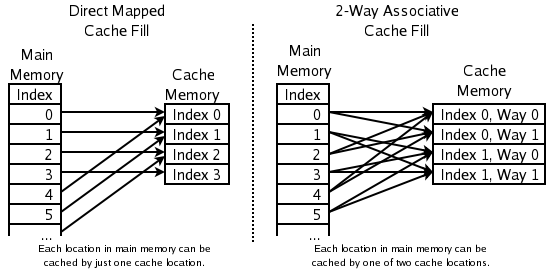
\includegraphics[width=0.8\textwidth]{images/cache-associative-fill-both.png}
\end{center}
主流的Intel是L1有32KB,8-Way,Cache Line是64bytes,于是有
\begin{enumerate}
    \item \text{cache line有32KB/64B=512条}
    \item \text{每一Way有512/8=64条cache line}
    \item \text{每一Way有64x64=4096bytes内存数据}
\end{enumerate}
为了方便索引地址,编码如下
\begin{itemize}
    \item \text{tag:每条cache line有24bit的物理地址}
    \item \text{index:每一Way的索引$2^6=64$,刚好索引每一Way的地址}
    \item \text{offset:每一Way中的cache line的偏移量}
\end{itemize}
\begin{center}
    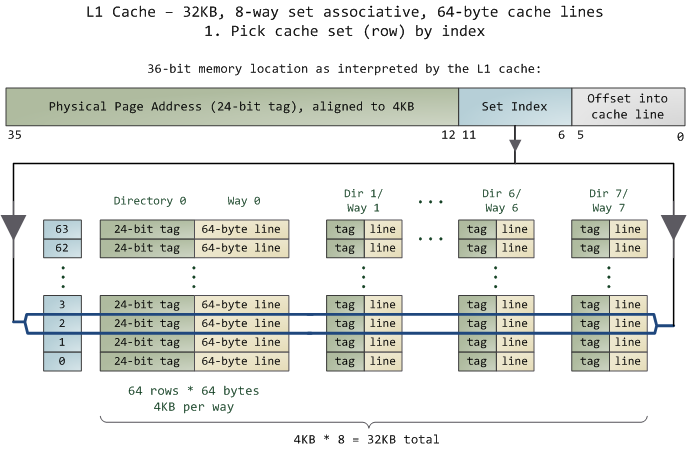
\includegraphics[width=0.8\textwidth]{images/L1CacheExample.png}
\end{center}
注意L1可以映射的内存地址是$2^36=64GB$,这样是解决了命中率的问题,还有Perfetching一些预测技术,可以一次性不止
64bytes的大小。

\subsection{一致性}

把数据从寄存器写出去产生的一致性问题,有两种策略

\begin{itemize}
    \item \text{Write Back, 只更新到cache,然后flush到内存上}
    \item \text{Write Through,更新到cache和内存上}
\end{itemize}

目前主流的还是Write Back策略,毕竟写入内存太耗时了。
现在假设一个数据X在CPU第0核的cache上更新了,其他核对于数据X也要更新,这就是一致性问题。
在CPU硬件层有两种方案:

\begin{itemize}
    \item [Directory] \text{存储全局信息,更新时同时检查哪些需要更新}
    \item [Snoopy] \text{以总线技术,类似广播形式,更新到所有的cache中的数据}
\end{itemize}

Directory属于中心式,会有性能瓶颈,目前都使用Snoopy总线设计方案。实现这些细节需要一些协议.

\subsubsection{MESI}

表示Modified已修改,Exclusive独占的,Shared共享的,Invalid无效的。

\begin{center}
    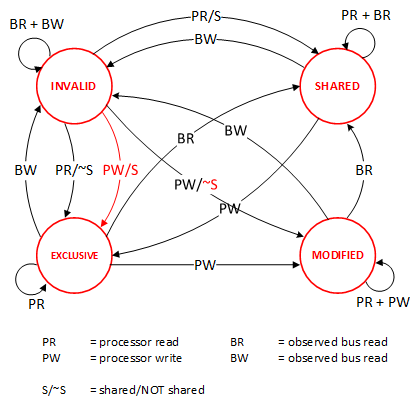
\includegraphics[width=0.8\textwidth]{images/MESI.png}
\end{center}

\begin{tabular}{|c|c|c|c|c|}
    \hline
    \hbox{当前操作} & CPU0 & CPU1 & Memory &  \hbox{说明} \\ \hline
    \hbox{1) CPU0 read(x)} & \hbox{x=1(E)} & & \hbox{x=1} & \hbox{只有一个CPU,状态是Exclusive} \\ \hline
    \hbox{2) CPU1 read(x)} & \hbox{x=1(S)} & \hbox{x=1(S)} & \hbox{x=1} & \hbox{两个CPU读取,状态为Shared} \\ \hline
    \hbox{3) CPU0 write(x,9)} & \hbox{x=9(M)} & \hbox{x=1(I)} & \hbox{x=1} & \hbox{变量改变,CPU0是Modified,CPU1是Invalid} \\ \hline
    \hbox{4) flush to memory} & \hbox{x=1(E)} & \hbox{x=1(E)} & \hbox{x=9} & \hbox{状态不变} \\ \hline
    \hbox{5) CPU1 read(x)} & \hbox{x=9(S)} & \hbox{x=9(S)} & \hbox{x=9} & \hbox{变量同步更新,状态为Shared} \\ \hline
\end{tabular}

AMD使用是MOESI,Intel使用的是MESIF。

\subsubsection{MOESI}

Owner宿主

\subsubsection{MESIF}

Forward


